\documentclass{article}
% \usepackage{xeCJK}
\usepackage{amsmath}
\usepackage{amssymb}
\usepackage{mathrsfs}
\usepackage{xcolor}
\usepackage{bm}
\usepackage{hyperref}
\usepackage{graphicx}
\usepackage{subcaption}
\usepackage{float}
\usepackage{csquotes}
\usepackage{multicol}
\usepackage[ruled,linesnumbered]{algorithm2e}

\bibliographystyle{plain}
\setlength{\parindent}{2em}
\usepackage{geometry}
\geometry{a4paper, left=2.54cm, right=2.54cm, top=3.18cm, bottom=3.18cm}

% 设置文章行距
% \renewcommand{\baselinestretch}{1.5}

% define reference format
\hypersetup{
    colorlinks=true,
    linkcolor=blue,
    urlcolor=blue,
    citecolor=blue,
    linkbordercolor=white
}

\title{\textbf{Enhancement of Demixing in Swarmalators with Inter-chiral Frustration}}
\author{Yichen Lu}

\begin{document}

\maketitle

\tableofcontents

\ \newline
\color{red}
    * All red parts are the methods that were tired but did not work.
\color{black}

\section{\label{sec:model}The Model}

Swarmalators have a spatial position $\mathbf{r}_i=\left( x_i, y_i \right)$ and an internal phase $\theta_i$ which evolve according to equations:
\begin{subequations} 
    \label{eq:totalDynamicsMeanField}
    \begin{align}
        \dot{\mathbf{r}}_i&=v\mathbf{p}\left( \theta _i \right)\;\label{eq:dotR},
        \\
        \dot{\theta}_i&=\omega _i+\frac{K}{\left| A_i \right|}\sum_{j\in A_i}{\left[ \sin \left( \theta _j-\theta _i+\alpha _{ij} \right) -\sin \alpha _{ij} \right]}\;\label{eq:dotTheta},
    \end{align}
\end{subequations}
for $i=1,2,\ldots,N$. Here in Eq.~(\ref{eq:dotR}), $\mathbf{p}\left( \theta \right) =\left( \cos \theta ,\sin \theta \right)$, which means each swarmalator rotates with a constant speed $v$ in the direction of its instantaneous phase $\theta_i (t)$. As per Eq.~(\ref{eq:dotTheta}), the sum runs over neighbors within a coupling radius $d_0$ around swarmalator $i$:
\begin{equation}
    A_i\left( t \right) =\left\{ j\mid \left| \mathbf{r}_i\left( t \right) -\mathbf{r}_j\left( t \right) \right|\leqslant d_0 \right\} \;,
\end{equation}
$K$ is the coupling strength, and $\omega_i$ is the natural frequency of the $i$-th swarmalator. 
This means that a swarmalator will rotate with the angular velocity $|\omega_i |$ in the absence of mutual coupling ($K=0$), and the sign of $\omega_i$ represents the direction of rotation, namely, the tribute of the chirality of the $i$-th swarmalator. A positive (negative) chirality ($\omega$) describes the counterclockwise (clockwise) rotations of the swarmalator in space. 
We will study swarmalators including two types of chiralities with both positive and negative natural frequencies uniformly distributed in two symmetric regimes as 
\begin{equation}
    g_U^{D}\left( \omega ;\mu,\sigma\right) 
    =\frac{1}{2}\left [
    g_U\left( \omega ;-\mu,\sigma\right) + 
    g_U\left( \omega ; \mu,\sigma\right) \right ].
    \label{eq:uniform2}
\end{equation}
where $g_U\left( \omega ;\mu ,\sigma \right)$ is the uniform distribution:
\begin{equation}
    g_U\left( \omega ;\mu ,\sigma \right) =\begin{cases}
	\frac{1}{\sigma},&		\omega _{\min}\leqslant \omega \leqslant \omega _{\max}\\
	0,&		\mathrm{otherwise}\\
\end{cases}\;.
\label{eq:uniform}
\end{equation}
Here $\sigma = \omega_{\max}-\omega _{\min}$ is the natural-frequency span, and $\mu = (\omega_{\max}+\omega _{\min})/2$ is the average.

Additionally, $\alpha_{ij}$ is the phase frustration between two neighboring swarmalators, which is defined as:
\begin{equation}
    \alpha _{ij}=\begin{cases}
        \alpha _0,&		\omega _i\omega _j<0\\
        0,&		\omega _i\omega _j\geqslant 0\\
    \end{cases}
\end{equation}
When $\alpha_0=0$, the dynamics reduces to the normal chiral model \cite{LU2025115794}. 
The counter term $\sin\alpha_{ij}$ is introduced to ensure that frustration only interferes with the inter-chiral coupling without changing the sign of natural frequency. 

Some order parameters can be introduced to measure the level of spatiotemporal coordination among swarmalators and distinguish the different collective states of the system. 
Firstly, an order parameter to measure the chiral demixing among swarmalators can be defined as:
\begin{equation}
    S\left( t \right) =\frac{1}{N}\sum_{i=1}^N{\frac{\sum_{j\in A_i}{H\left( \omega _i\omega _j \right)}}{\left| A_i\left( t \right) \right|}}\;,
\end{equation}
where $H\left( x \right) =\left( x>0 \right)$ is the Heaviside step function. $S\left( t \right)$ is the fraction of the pairs of neighboring swarmalators with the same chirality. When $S\left( t \right)=1$, all the neighboring pairs of swarmalators have the same chirality, and the system is in a completely phase-separated state. When $S\left( t \right)< 1$, the system is in a mixed state.

Except for measuring the demixing degree, an order parameter to measure the degree of the complete demixing can be defined as:
\begin{equation}
    M\left( t \right) =\frac{1}{N}\sum_{i=1}^N{H\left[ \sum\nolimits_{j\in A_i}^{}{H\left( -\omega _i\omega _j \right)} \right]}\;.
\end{equation}
$M\left( t \right)$ is the fraction of swarmalators that have neighbors with different chirality. When $M\left( t \right)=0$, all the swarmalators are in a completely phase-separated state. When $M\left( t \right)> 0$, the system is in a mixed state. Obviously, $M$ describes the qualitative nature of the mixing, while $S$ describes the quantitative nature.

The above order parameters measure the chiral demixing from the perspective of the spatial distribution of the swarmalators. 
The coordination of the internal phases can also be quantified to describe the demixing of the system. Firstly, a usual order parameter to measure the phase synchronization of the system can be defined as: 
\begin{equation}
    Z\left( t \right) =R\left( t \right) \mathrm{e}^{\mathrm{i}\psi \left( t \right)}=\frac{1}{N}\sum_{j=1}^N{\mathrm{e}^{\mathrm{i}\theta _j\left( t \right)}}\;,
\end{equation}
where $\textrm{i}=\sqrt{-1}$. The degree modulus $R(t)=\left|Z(t)\right|$ is the absolute value of the mean of the complex numbers $e^{\textrm{i}\theta _i}$, which can be interpreted as the absolute value of the mean normalized velocity of all swarmalators. When $R\approx 1$, swarmalators are fully phase synchronized, and when $R\approx0$, swarmalators are phase incoherent.
When the system is in a mixed state, the order parameter $R$ remains constant in the long run, while for the phase-separated state, $R$ will fluctuate over time. These behaviors can be quantified by the maximum and minimum values of $R$ in a certain time window:
\begin{subequations}
    \begin{align}
        R_{\max}&=\max_{t\in W} \left\{ R\left( t \right) \right\} 
        \\
        R_{\min}&=\min_{t\in W} \left\{ R\left( t \right) \right\} 
    \end{align}
\end{subequations}
where $W=\left[ T-h,T+h \right]$ is a time window that is long enough to cover the transient and steady states of the system. When $R_{\max}=R_{\min}\approx1$, the system is in a mixed state, and when $R_{\max}\neq R_{\min}$, the system is phase-separated. 

We conducted numerical simulations to investigate the performance and characteristics of our system under various conditions.
For simplicity, we assume that swarmalators are initially distributed uniformly in a two-dimensional $L\times L$ square with periodic boundary conditions.
All the numerical simulations of the model Eq.~(\ref{eq:totalDynamicsMeanField}) were run on Python using Euler integration with box size of $L=7$, population sizes of $N=1000$, natural-frequency span $\sigma=1$, minimal absolute value of frequencies $\omega_{\min}$ in $\left[ 10^{-3}, 3 \right]$, and coupling radius of $d_0=1$. 
Unless otherwise stated, each data point of order parameters was collected by averaging last 1000 time steps of the simulation to discard the transients.


\begin{figure*}
    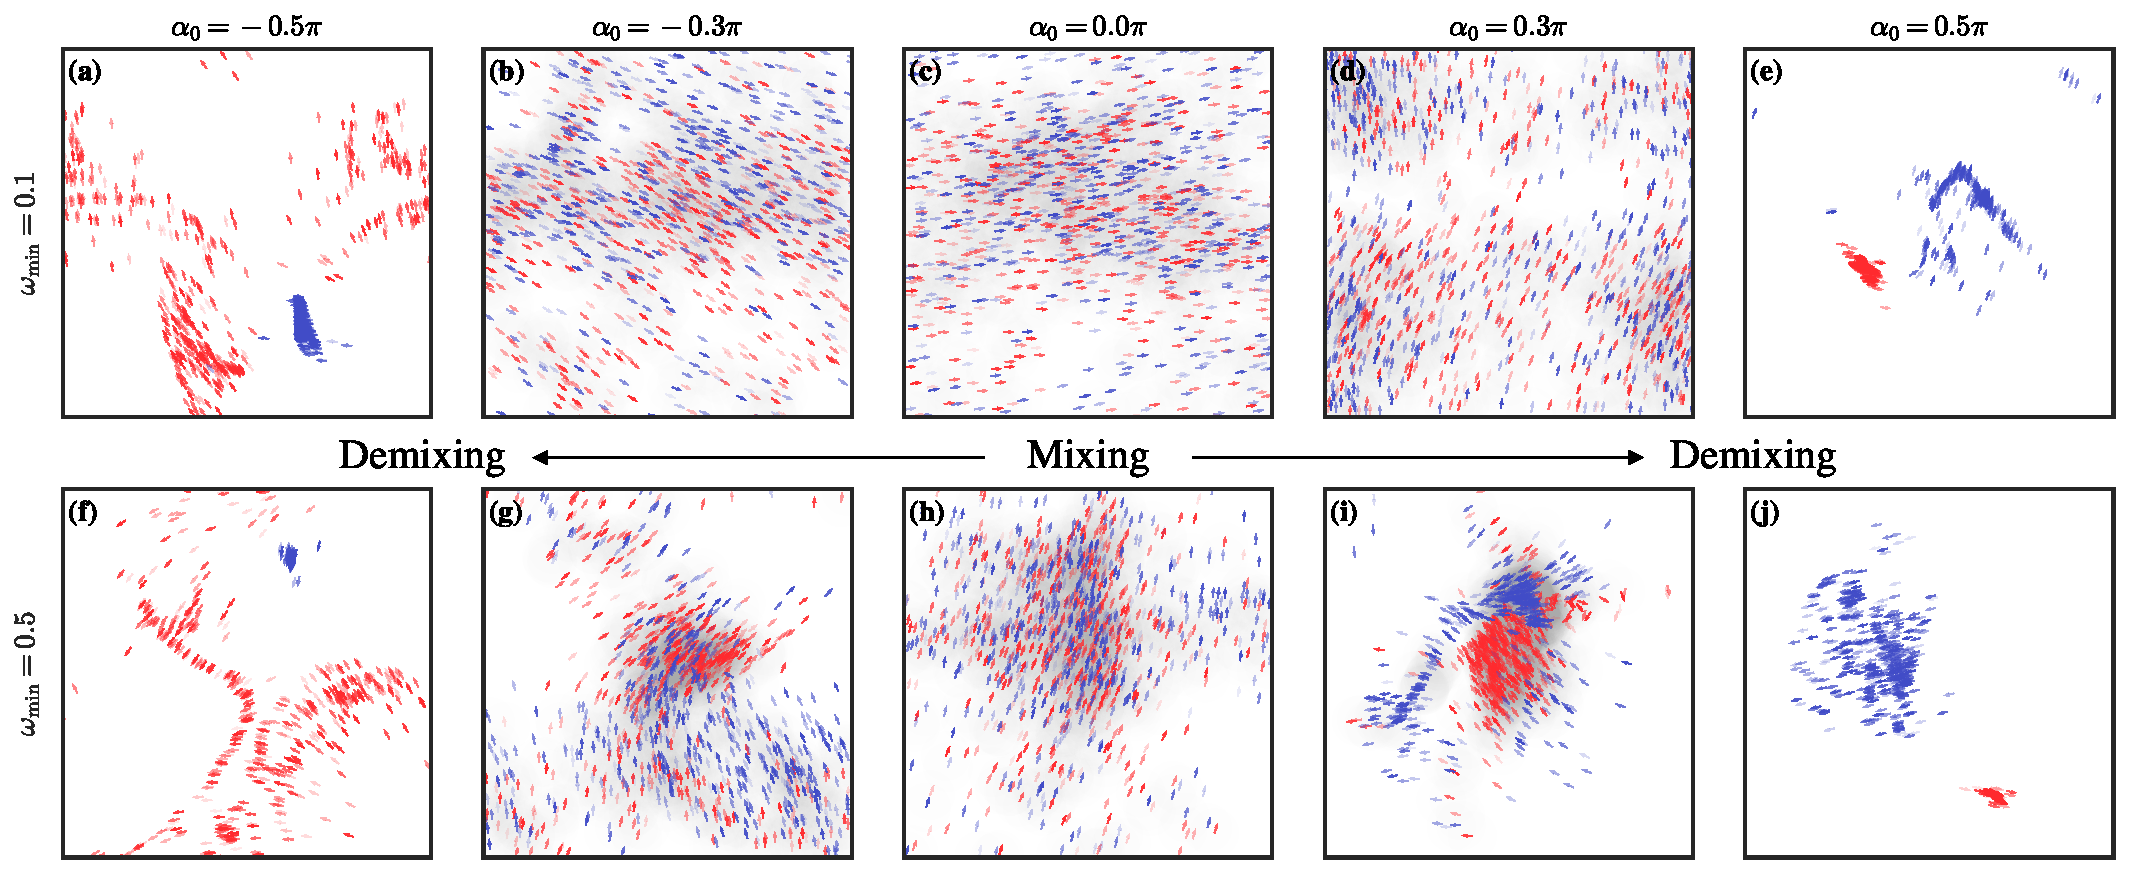
\includegraphics[width=\textwidth]{./figs/snapshots.pdf}
    \caption{
        \label{fig:snapshots} Snapshots of the spatial distribution for different minimal frequency $\omega_{\min}$ and phase frustration $\alpha_0$. 
        Two types of chiral swarmalators are represented by red ($\omega_i$>0) and blue ($\omega_i$<0) arrows, respectively.
        The position and direction of the arrows represent the spatial position and phase of the swarmalators, respectively. The swarmalators with neighbors of opposite chirality are marked with a gray background.
    }
\end{figure*}

\begin{figure*}
    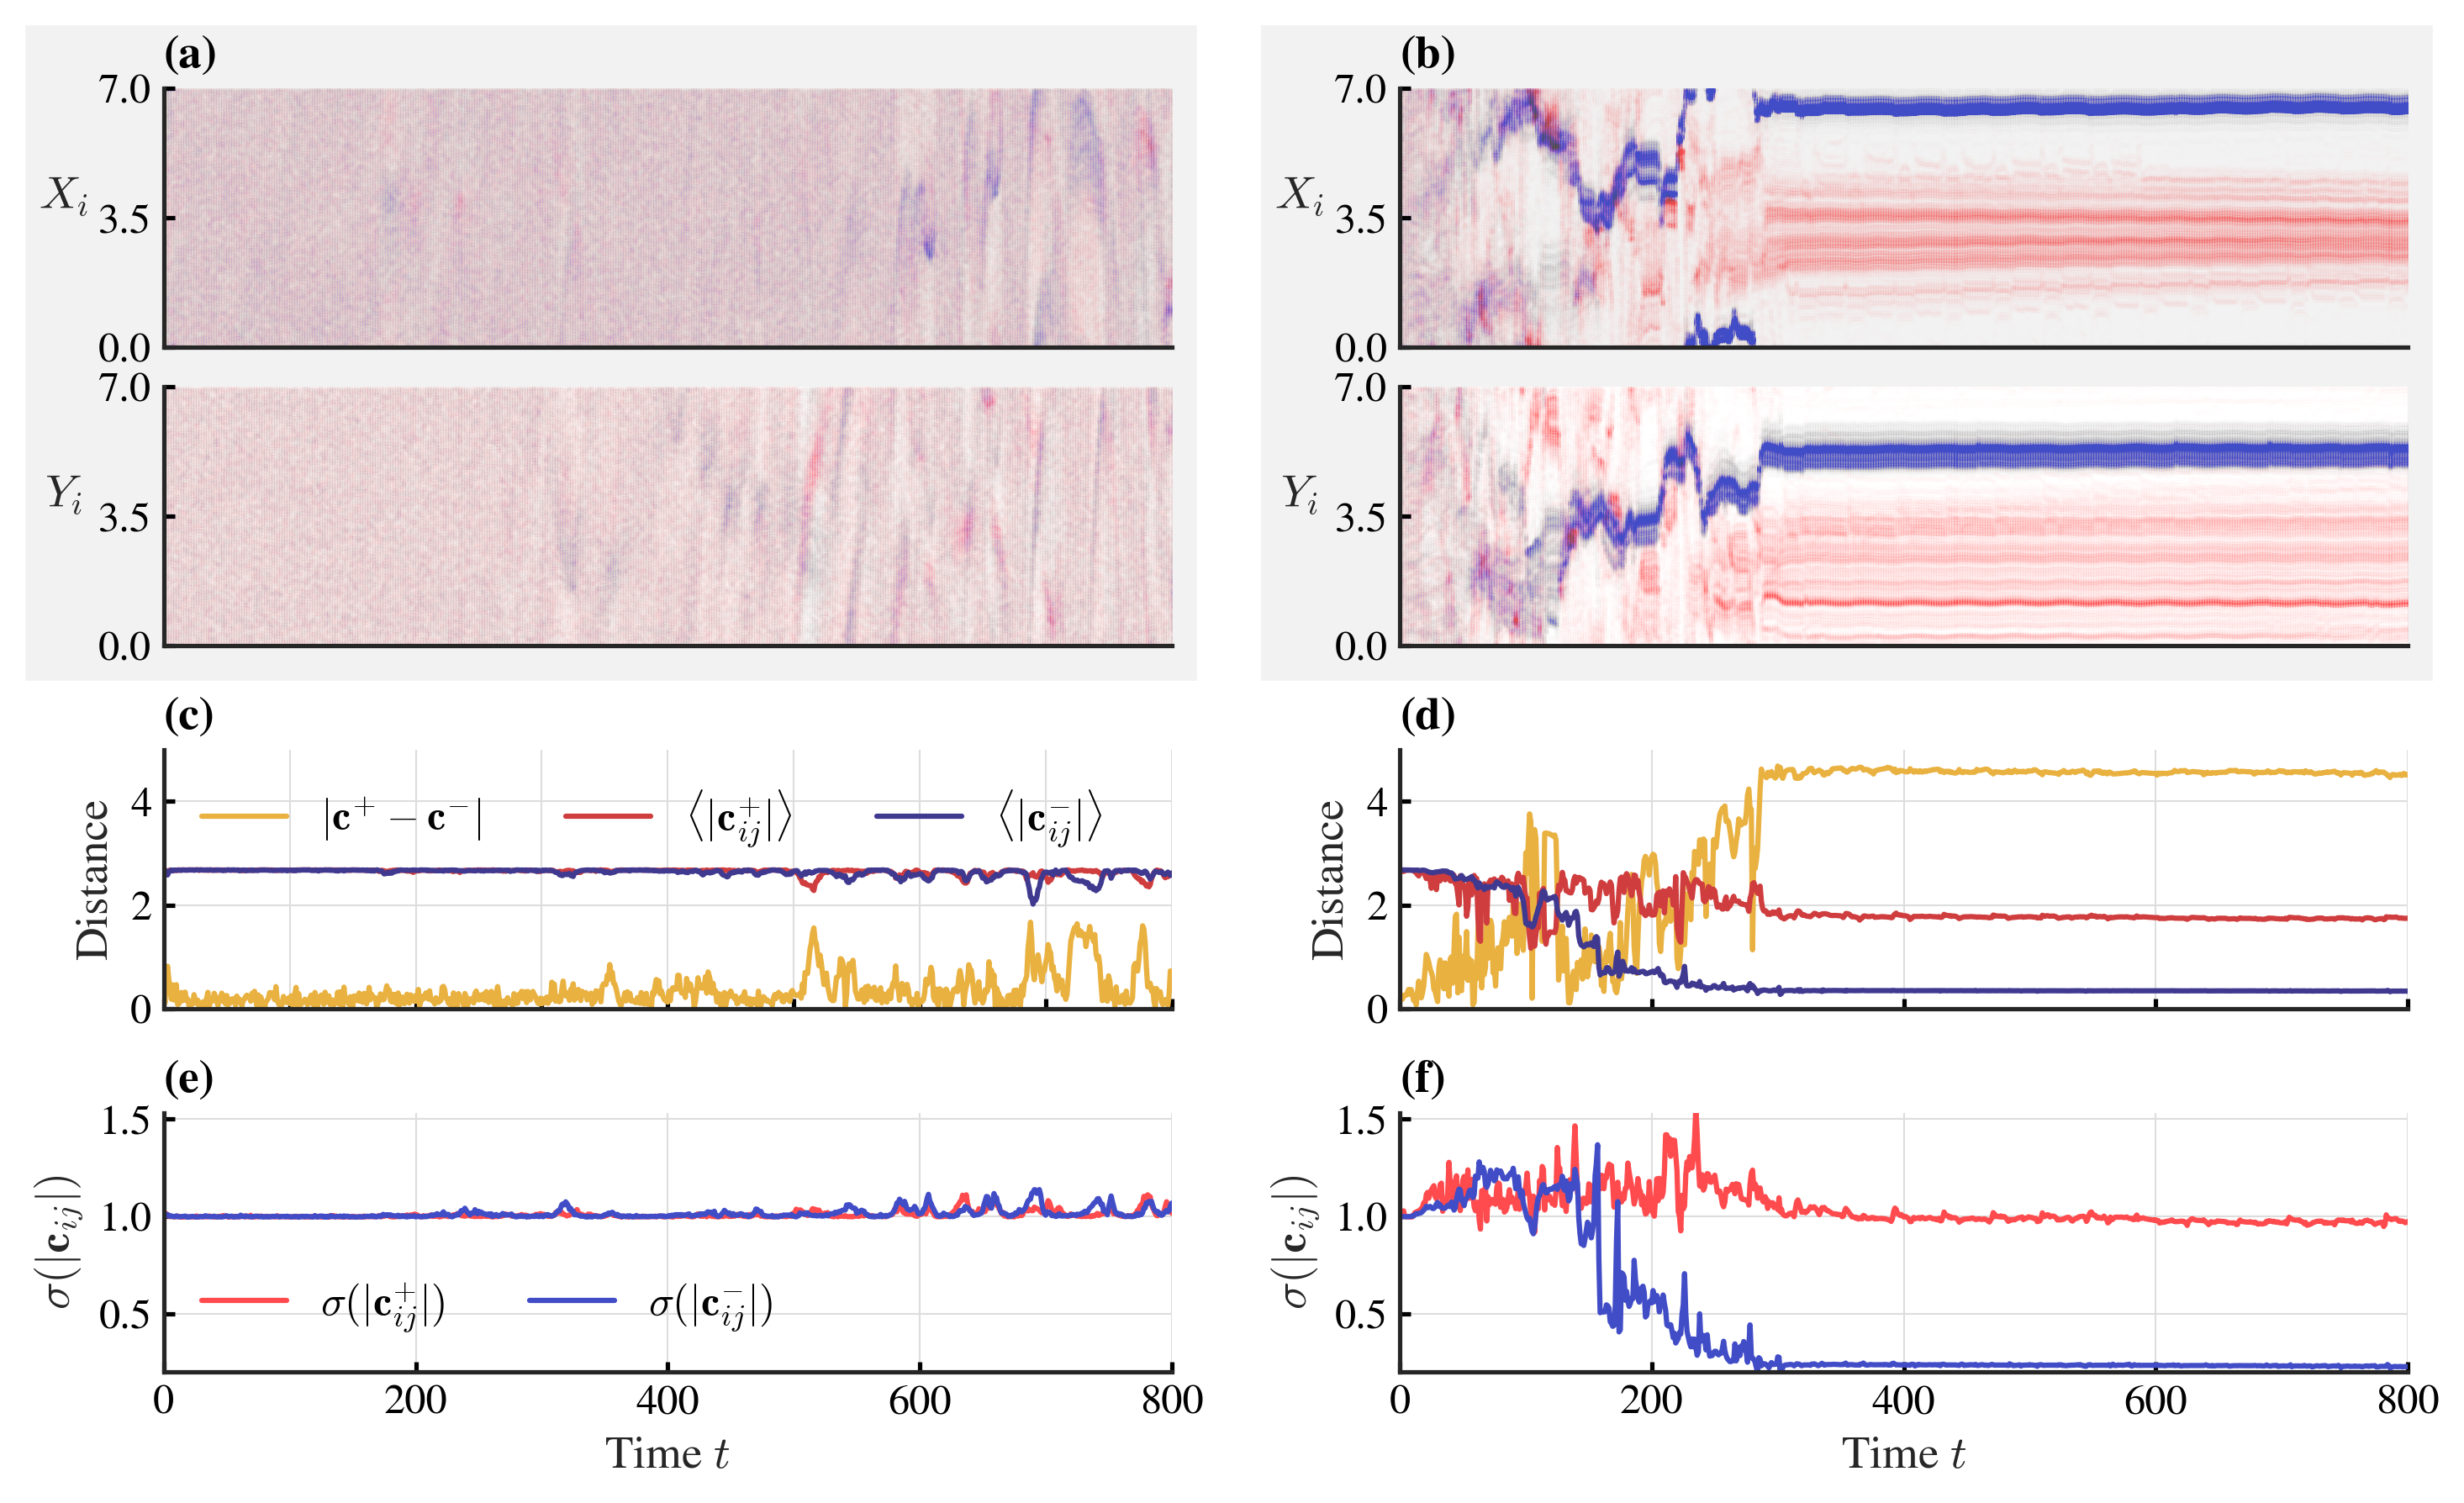
\includegraphics[width=\textwidth]{./figs/centersScatterXY.png}
    \caption{
        \label{fig:centersScatterXY} 
        Demixing behaviors of the system with different phase frustrations $\alpha_0$: \textbf{(a, c, e)}, $\alpha_0=0$; \textbf{(b, d, f)}, $\alpha_0=-0.5\pi$ and $\omega_{\min}=1.1$.
        \textbf{(a, b)}, scatter plot of the instantaneous rotational centers of swarmalators. The color of the dots denotes the corresponding natural frequency.
        \textbf{(c, d)}, the time evolution of the distance between like/opposite chirality centers.
        \textbf{(e, f)}, the time evolution of the standard deviation of the distance between like chirality centers. 
    }
\end{figure*}

\begin{figure*}
    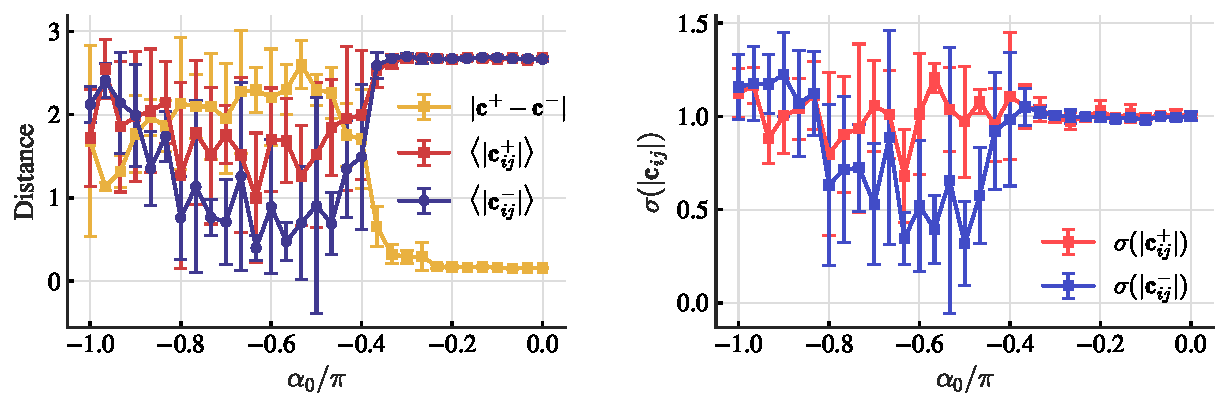
\includegraphics[width=0.85\textwidth]{./figs/distancesVsAlpha.pdf}
    \caption{
        \label{fig:distancesVsAlpha} 
        The mean and standard deviation of the distance between centers versus phase frustration $\alpha_0$.
        \textbf{(a)}, the distance between centers of neighboring swarmalators versus $\alpha_0$.
        \textbf{(b)}, the standard deviation of distance between centers of neighboring swarmalators versus $\alpha_0$.
        All data points are averaged over different initial conditions for $\omega_{\min}=10^{-3}$. (error-bars representing the standard deviation).
    }
\end{figure*}

\section{\label{sec:behaviors}Frustration-enhanced demixing}

Swarmalators with inter-chiral frustration can significantly enhance the chiral demixing of the system, both during the transient and in the steady state. 
The spatial distribution of the swarmalators is shown in Fig.~\ref{fig:snapshots} by modulating the minimal frequencies $\omega_{\min}$ and phase frustrations $\alpha_0$.
Mixing state is observed when the minimal frequency $\omega_{\min}l\ll1$ and phase frustration $\left|\alpha_0\right|\ll 1$ (see the snapshots (b-d, h) of Fig.~\ref{fig:snapshots}), as the phase frustration is not strong enough to interfere with the inter-chiral coupling. 
When the minimal frequency $\omega_{\min}$ is increased, the difference in natural frequencies between two chiral substances becomes significant, and the system will phase separate into two clusters with the same chirality, which can be regarded as the self-organized phase separation of the system. 
As an external interference, the phase separation is more pronounced when the phase frustration $\alpha_0$ is increased, as shown in the snapshots (a, e, f, j), and this effect can also be observed for extremely small frequency differences, which is illustrated in the first row of Fig.~\ref{fig:snapshots}. Additionally, the sign of the frustration, $\text{sgn}\alpha_0$, can also affect the spatial scale of the clusters.
When the phase frustration $\alpha_0$ is positive, clusters with positive chirality are more compact, whereas clusters with negative chirality tend to be more dispersed, as illustrated in snapshots (a, f). In contrast, when the phase frustration $\alpha_0$ is negative, the scale of two chirality clusters is reversed, as shown in snapshots (e, j).


To further investigate the chiral demixing of the system, we introduced the instantaneous rotational centers $\mathbf{c}_i\left(t\right)=\left(X_i\left(t\right), Y_i\left(t\right)\right)$, which is given by
\begin{equation}
    \begin{aligned}
        X_i\left( t \right) &=x_i\left( t \right) -\frac{\upsilon}{\dot{\theta}_i\left( t \right)}\sin \theta _i\left( t \right) ,\\
        Y_i\left( t \right) &=y_i\left( t \right) +\frac{\upsilon}{\dot{\theta}_i\left( t \right)}\cos \theta _i\left( t \right) .\\
    \end{aligned}
\end{equation}
By starting from uniform initial conditions, the instantaneous rotational centers of the swarmalators are shown in Fig.~\ref{fig:centersScatterXY}(a, b) for the minimal frequency $\omega_{\min}=1.1$ and phase frustrations $\alpha_0=0, -0.5\pi$, respectively.
When $\alpha_0=0$, the two chiralities are mixed together, and the centers are distributed uniformly in the space, as demonstrated in Fig.~\ref{fig:centersScatterXY}(a). 
When $\alpha_0=-0.5\pi$, it is clearly shown that swarmalators with the same chirality converge into one cluster with increasing time, while swarmalators with opposite chirality exhibit a clear separating effect, i.e., centers with dual chiralities labeled in red and blue approach to different ranges, and the scale of the positive and negative chirality clusters is relatively dispersed and compact, as illustrated in Fig.~\ref{fig:centersScatterXY}(b), which is consistent with the snapshots in Fig.~\ref{fig:snapshots}(a, f).
Some further quantitative analysis is conducted to describe the demixing process of the system. Firstly, the most intuitive metric is the distance between mean centers of two chiralities:
\begin{equation}
    \left| \mathbf{c}^+-\mathbf{c}^- \right|=\left| \frac{1}{N_c}\sum_{i=1}^{N_c}{\mathbf{c}_{i}^{+}}-\frac{1}{N_c}\sum_{i=1}^{N_c}{\mathbf{c}_{i}^{-}} \right|\;,
\end{equation}
where the notation $\pm$ denotes the positive and negative chiralities, respectively. From the opposite perspective, the mean distance between the centers of the same chirality can describe the compactness of the clusters:
\begin{equation}
     \langle \left| \mathbf{c} \right|_{ij}^{\pm} \rangle =\frac{2}{N_{c}^{2}}\sum_{i=1}^{N_c}{\sum_{j=1}^i{\left| \mathbf{c}_{i}^{\pm}-\mathbf{c}_{i}^{\pm} \right|}}\;,
\end{equation}
where $N_c=N/2$ is the number of swarmalators with the same chirality. 
As illustrated in Fig.~\ref{fig:centersScatterXY}(c, d), when $\alpha_0 = 0$, the distance between centers of both like and opposite chirality remains nearly constant. However, for $\alpha_0 = -0.5\pi$, there is a notable decrease in the distance between centers of negative chirality, while the distance between centers of different chiralities increases. This observation suggests a phase separation within the system. Furthermore, the standard deviation of the distances between centers of the same chirality,
\begin{equation}
    \sigma ( \left| \mathbf{c} \right|_{ij}^{\pm} ) =\sqrt{\frac{2}{N_{c}^{2}}\sum_{i=1}^{N_c}{\sum_{j=1}^i{\left( \left| \mathbf{c}_{i}^{\pm}-\mathbf{c}_{i}^{\pm} \right|-\left< \left| \mathbf{c} \right|_{ij}^{\pm} \right> \right) ^2}}}\;,
\end{equation}
can serve as a measure of cluster compactness, as depicted in Fig.~\ref{fig:centersScatterXY}(e, f). At $\alpha_0 = -0.5\pi$, the standard deviation of the distances between centers within negative chirality is significantly lower, indicating that these clusters are more compact.

\begin{figure*}
    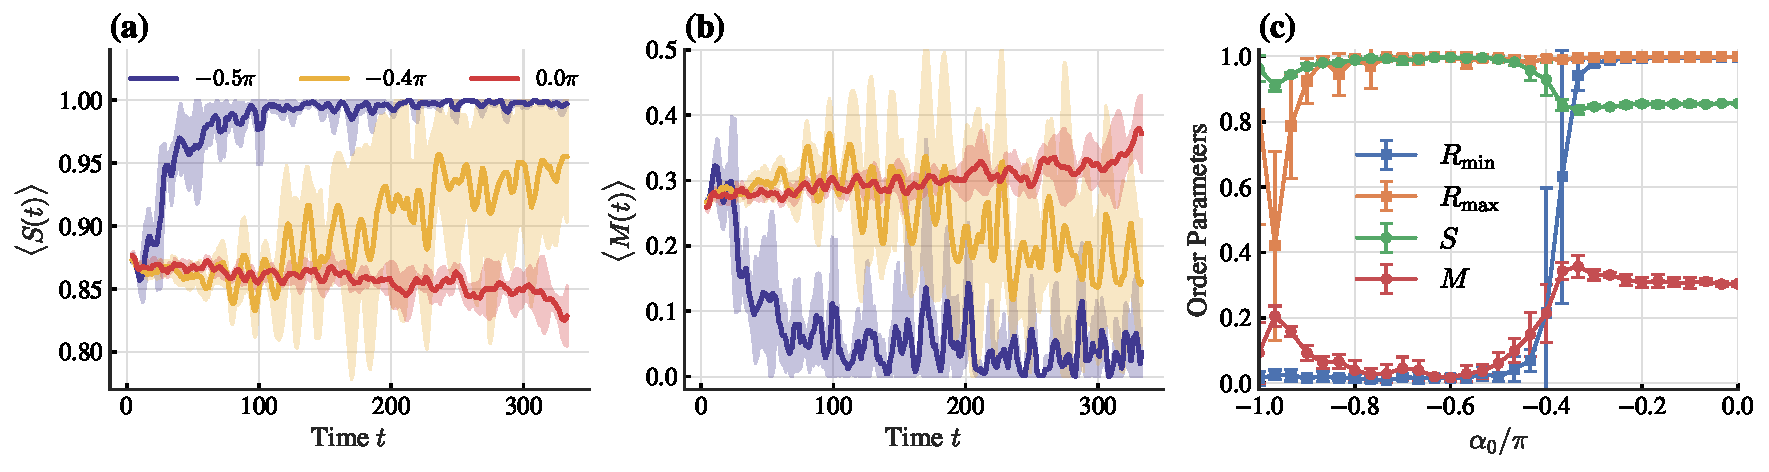
\includegraphics[width=\textwidth]{./figs/orderParameters.pdf}
    \caption{
        \label{fig:orderParameters} 
        \textbf{(a--b)}, time evolution of the order parameters $S$ and $M$ for different phase frustration $\alpha_0$, where \enquote{$\langle\cdot\rangle$} denotes the average taken over the minimal frequency $\omega_{\min}\in\left[0.1, 0.5\right]$.
        \textbf{(c)}, order parameters $S$, $M$, $R_{\max}$ and $R_{\min}$ versus $\alpha_0$ averaged over different initial conditions for $\omega_{\min}=10^{-3}$.
        (translucent bond and error-bars representing the standard deviation).
    }
\end{figure*}

In addition to characterizing the time-varying spatial distribution of the swarmalators, frustration-varying behaviors can also be observed in the distance between the centers, as shown in Fig.~\ref{fig:distancesVsAlpha} with $\omega_{\min}=10^{-3}$. Considering the symmetry in how $\text{sgn}\alpha_0$ influences model behavior, we only present the results for $\alpha_0\in\left[ -\pi, 0 \right]$. 
As evident in Fig.~\ref{fig:distancesVsAlpha}(a), with the increase of frustration strength $\left|\alpha_0\right|$, the distance between the centers of different chiralities initially is close to zero in the mixed state, and then bifurcates from zero and increases rapidly at $\alpha_0\approx -0.4\pi$, indicating the demixing of the system. Around $\alpha_0\approx -0.5\pi$, the distance between the centers of different chiralities reaches a maximum, and then decreases slightly with further increase of $\left|\alpha_0\right|$ until it reaches $-\pi$, where the demixing degree increases again for the phase coupling turning to the exact opposite direction. 
The distances between the centers of the same chirality also exhibits an opposite trend, which is consistent with the compactness of the clusters, where the negative cluster is more compact than the positive cluster. This is further confirmed by the standard deviation of the distances between the centers of the same chirality, as shown in Fig.~\ref{fig:distancesVsAlpha}(b). The standard deviation of the negative chirality decreases with the increase of $\left|\alpha_0\right|$, and reaches a minimum at $\alpha_0\approx -0.5\pi$, which is clearly lower than that of the positive chirality.

To quantify the level of chiral demixing, we calculated the order parameters $S$, $M$ to measure the fraction of neighboring pairs of swarmalators with the same chirality and the fraction of swarmalators that have neighbors with different chirality, respectively. Fig.~\ref{fig:orderParameters}(a, b) shows the time evolution of the order parameters $S$ and $M$ for different phase frustrations $\alpha_0$, where \enquote{$\langle\cdot\rangle$} denotes the average taken over the minimal frequency $\omega_{\min}\in\left[0.1, 0.5\right]$. 
When $\alpha_0=0$, the system is in a mixed state, and the order parameters $S$ and $M$ decreases and increases slightly over time, respectively. 
For $\alpha_0=-0.4\pi$, the system undergoes a phase transition from the mixed state to the demixing state, where the order parameters $S$ and $M$ exhibit a significant increase and decrease, respectively.
While for the most effective frustration $\alpha_0=-0.5\pi$, the order parameters $S$ and $M$ vary rapidly and achieve a steady state quickly, indicating that the system is in a completely phase-separated state, where the order parameters $S$ and $M$ reaches their maximum and minimum values, respectively.

Homoplastically, the order parameters $S$, $M$, $R_{\max}$ and $R_{\min}$ versus $\alpha_0$ are shown in Fig.~\ref{fig:orderParameters}(c). The trend of the order parameters $S$ and $M$ is consistent with the results of the time evolution, where the order parameter $S$ increases and $M$ decreases with the increase of $\left|\alpha_0\right|$ until they reach their maximum and minimum values, respectively. After that, the order parameters $S$ and $M$ decrease and increase slightly, respectively, as the degree of demixing weakens. On the other hand, the order parameters $R_{\max}$ and $R_{\min}$ provide an ultrasound confirmation with $S$ and $M$, where $R_{\max}$ and $R_{\min}$ are equal to 1 for the weak frustration, and then bifurcate to different values for the stronger frustration, which indicates the partial locking of the phases in the system.
Consistent with the trend of $S$ and $M$, the difference between $R_{\max}$ and $R_{\min}$ decreases with the increase of $\left|\alpha_0\right|$ after passing the maximum point, and then increases again when $\alpha_0$ touches $-\pi$.

\begin{figure*}
    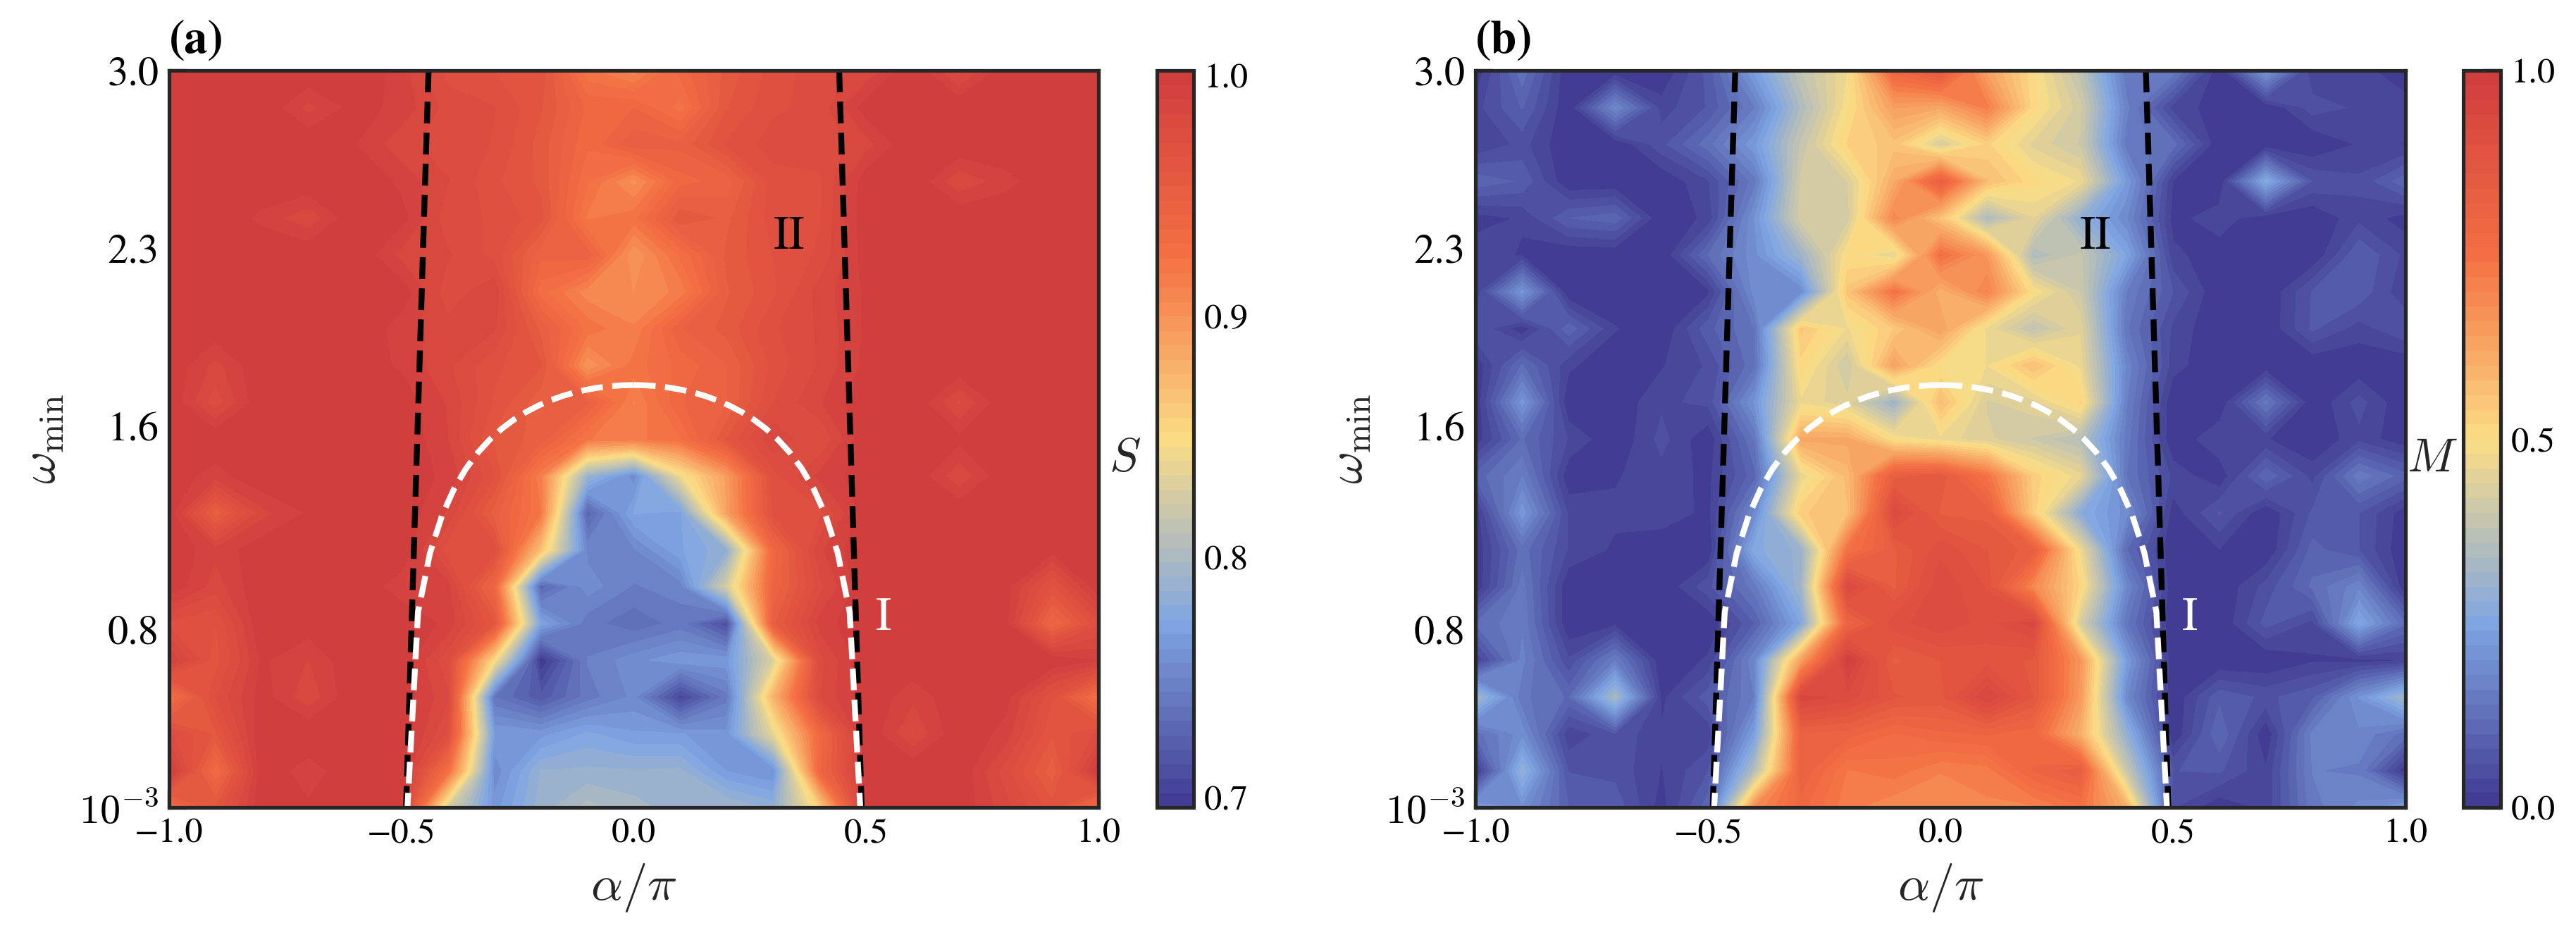
\includegraphics[width=\textwidth]{./figs/phaseDiagram.png}
    \caption{
        \label{fig:phaseDiagram} 
        Heatmaps for order parameters $S$, $M$ across the phase diagram of $(\alpha_0, \omega_{\min})$ with the critical demixing frustration $\alpha_{c}$ (black dashed line) and the critical swarming frustration $\alpha_{s}$ (white dashed line).
        Different colors describe the amplitudes of different order parameters.
    }
\end{figure*}

\section{\label{sec:phaseDiagram}Phase diagrams and theoretical approximation}

To construct the phase diagram of the system, we calculated the order parameters $S$, $M$ across the phase diagram of $(\alpha_0, \omega_{\min})$ and drive the critical frustrations for the enhancement of chiral demixing, as shown in Fig.~\ref{fig:phaseDiagram}.
The order parameters $S$ and $M$ are color-coded to represent the amplitudes of the order parameters.
The dashed lines labeled I and II represent the critical frustrations $\alpha_{c}$ and $\alpha_{s}$, respectively. Line I is the critical frustration for the enhancement of swarming,  and line II is for the chiral demixing. It can be seen that the two critical lines can be well manifested in the phase diagram, where the order parameters $S$ and $M$ exhibit a significant change across the critical lines.

The phase diagram shows that the system is in a mixed state when $\omega_{\min}\ll1$ and $\left|\alpha_0\right|\ll1$, where the order parameters $S$ and $M$ are close to 0.7 and 1, respectively, corresponding to the region A in Fig.~\ref{fig:phaseDiagram}.  
When the minimal frequency $\omega_{\min}$ surmounts the critical line $\alpha_s^{-1}(\omega_{\min})$ (white dashed line), the system will phase separate into two clusters with the same chirality, and the order parameters $S$ increase obviously, while the order parameters $M$ decrease but remain close to 1, which can be seen by comparing the regions B in sub-figures (a) and (b) of Fig.~\ref{fig:phaseDiagram}, because the phase separation strengthens the demixing degree, but the coupling between the two chiralities is still strong. 
When the phase frustration $\alpha_0$ exceeds the critical line $\alpha_c(\omega_{\min})$ (black dashed line), the system will achieve the complete demixing state, where the order parameters $S$ and $M$ reach their maximum and minimum values, respectively, as shown in the region C in Fig.~\ref{fig:phaseDiagram}. As the frustration continues to increase, the order parameters $S$ and $M$ decrease and increase slightly, respectively, as the degree of demixing weakens.

The dynamics of the system (\ref{eq:totalDynamicsMeanField}) in the mixing state can be abstracted as a synchronization problem in multilayer networks for its spatially uniform distribution. Therefore, for the symmetry of the spatial distribution and the mean-field coupling, each local subset of connected swarmalators can be regarded equivalently as a group of swarmalators in mean-field coupling.
This problem can be described by the following equations:
\begin{equation}
    \label{eq:multiLayer}
    \begin{aligned}
        \dot{\theta}_{i}^{\pm}=&\omega _{i}^{\pm}+\frac{K}{N}\sum_{j=1}^{_{N_c}}{\sin \left( \theta _{j}^{\pm}-\theta _{i}^{\pm} \right)}\\
        &+\frac{K}{N}\sum_{j=1}^{_{N^{\mp}}}{\left[ \sin \left( \theta _{j}^{\mp}-\theta _{i}^{\pm}+\alpha _0 \right) -\sin \alpha _0 \right]}\;,
    \end{aligned}
\end{equation}
where $N_c=N/2$ is the numbers of swarmalators with positive and negative chirality, respectively. 
Each layer $\pm$ represents the swarmalators with the same chirality, and the second, third terms in Eq.~(\ref{eq:multiLayer}) describe the intralayer and interlayer interactions, respectively.

Let $\theta _{i}^{\pm}\left( t \right) =\theta ^{\pm}$ and introduce $\Delta \theta=\theta^{+}-\theta^{-}$, $\Delta \omega=\mu^{+}-\mu^{-}$, the phase locking dynamics of two layers can be described by the following equations:
\begin{equation}
    \label{eq:phaseLocking}
    \Delta \dot{\theta}=\Delta \omega -K\sin \left( \theta ^+-\theta ^- \right) \cos \alpha _0\;.
\end{equation}
When $K^{-1}\Delta \omega \leqslant 1$, Eq.~(\ref{eq:phaseLocking}) has fixed points solutions $\Delta \theta =\arcsin \left( K\sin \alpha _0\Delta \omega \right)$, which means the two layers are phase-locked. 
When $K^{-1}\Delta \omega > 1$, the two layers are not phase-locked, and the phase difference $\Delta \theta$ will drift with time. Therefore, the critical frustration $\alpha _0$ can be driven by the natural frequency difference $\Delta \omega$ and coupling strength $K$ as
\begin{equation}
    \label{eq:criticalFrustration}
    \alpha _c=\arccos \frac{\left| \Delta \omega \right|}{K}\;.
\end{equation}
The critical line of the demixing is shown in Fig.~\ref{fig:phaseDiagram}. The critical frustration $\alpha _0$ descends with the minimal natural frequency $\Delta \omega$ increasing until the fixed point solution of Eq.~(\ref{eq:phaseLocking}) is absent.

Ref.~\cite{LU2025115794} gives another critical frustration $\alpha _s$ for the swarming transition, which is the critical frustration for the swarming transition:
\begin{equation}
    \label{eq:criticalFrustrationSwarming}
    \alpha _s=\mathrm{arc}\cos \frac{2\pi d_0\left| \Delta \omega \right|}{K\left( 2\beta d_0-2r_d\sin \frac{\beta}{2} \right)}\;,
\end{equation}
with the terms being
\begin{equation}
    \begin{aligned}
        r_d&=\frac{L}{\sqrt{2}}-d_0-2r_o\;,\\
        \beta &=2\mathrm{arc}\cos \frac{r_{d}^{2}}{2d_0r_d}\;,\\
        r_o&=\frac{v}{\mu ^+}=-\frac{v}{\mu ^-}\;,\\
    \end{aligned}
\end{equation}


\begin{figure}
    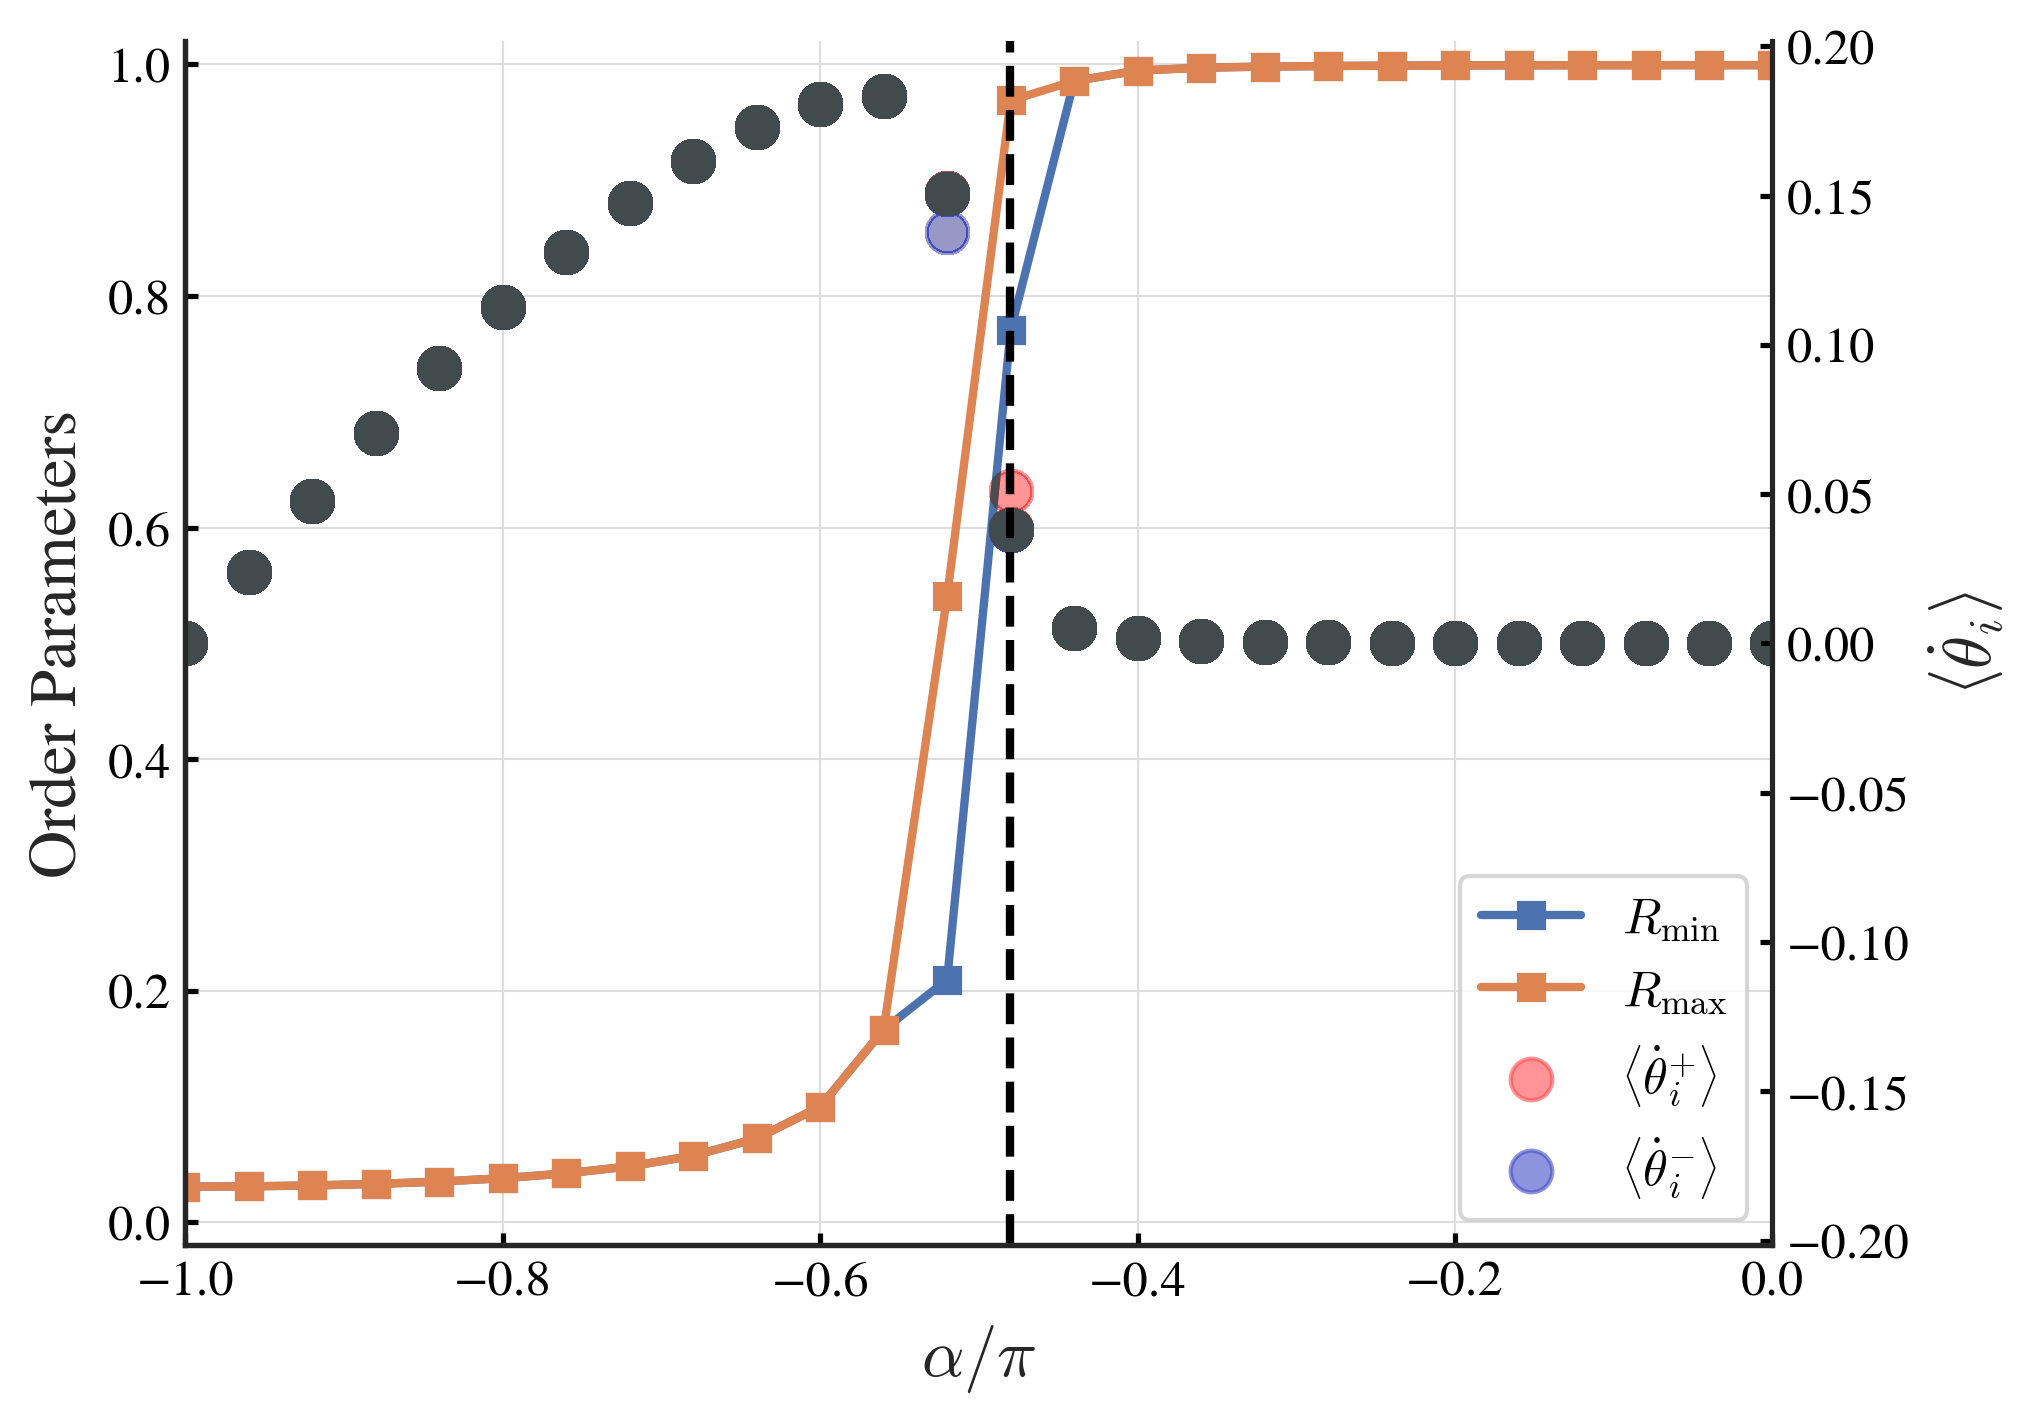
\includegraphics[width=0.49\textwidth]{./figs/SyncOPsAndRealFreq.png}
    \caption{
        \label{fig:SyncOPsAndRealFreq} 
        Heatmaps for order parameters $S$, $M$ across the phase diagram of $(\alpha_0, \omega_{\min})$ and the critical frustration $\alpha_{0c}$ (black dashed line). Different colors describe the amplitudes of different order parameters.
    }
\end{figure}


% #####################################################
\newpage
\color{red}
\subsection{OA Reduction}

To quantify the inter-layer coherence of the system, it is convenient to define the generalized complex-valued
order parameters, i.e.,
\begin{equation}
    \label{eq:orderParameter}
    Z^{\pm}\left( t \right) =R^{\pm}\left( t \right) \text{e}^{\text{i}\psi^{\pm}\left( t \right)}=\frac{1}{N}\sum_{j=1}^N{\text{e}^{\text{i}\theta _{j}^{\pm}\left( t \right)}}\;,
\end{equation}
where $n=1,2,\dots, N$, and $r^{\pm}\left( t \right)$, $\psi ^{\pm}\left( t \right)$ are the amplitudes and arguments of the $n$-order parameter.
Our starting point is to analyze the critical point for the pulsation of the order parameter.
In the thermodynamic limit $N\rightarrow \infty$, where $N^{\pm}\rightarrow \infty$. Then
Eq.~(\ref{eq:multiLayer}) gives rise to the continuity equations
\begin{equation}
    \label{eq:continuity}
    \frac{\partial \rho ^{\pm}}{\partial t}+\frac{\partial}{\partial \theta}\left( \rho ^{\pm}v^{\pm} \right) =0
\end{equation}
where $\rho ^{\pm}\left( \theta ,\omega ,t \right)$ is the probability density of oscillators in layer $\pm$ with phase $\theta$ at fixed frequency $\omega$ and $t$, it satisfies the normalization condition
\begin{equation}
    \label{eq:normalization}
    \int_{0}^{2\pi}{\rho ^{\pm}\left( \theta ,\omega ,t \right) \text{d}\theta} =1\;.
\end{equation}
Here, $v^{\pm}\left( \theta ,\omega ,t \right)$ is the velocity field, given by
\begin{equation}
    \begin{aligned}
        &v^{\pm}\left( \theta ,\omega ,t \right) =\omega -\frac{K}{2}\sin \alpha _0\\
        &+\frac{K}{2}\int{\sin \left( \theta ^{\prime}-\theta \right) \rho ^{\pm}\left( \theta ^{\prime},\omega ^{\prime},t \right) \text{d}\theta ^{\prime}\text{d}\omega ^{\prime}}\\
        &+\frac{K}{2}\int{\sin \left( \theta ^{\prime}-\theta +\alpha _0 \right) \rho ^{\mp}\left( \theta ^{\prime},\omega ^{\prime},t \right) \text{d}\theta ^{\prime}\text{d}\omega ^{\prime}}\;.\\
    \end{aligned}
\end{equation}
Correspondingly, the 1-order parameter defined in Eq.~(\ref{eq:orderParameter}) in the thermodynamic limit reads
\begin{equation}
    \label{eq:continuityZ}
    z^{\pm}\left( t \right) =\int_{-\infty}^{+\infty}{g^{\pm}(\omega)\int_0^{2\pi}{\text{e}^{\text{i}\theta}\rho ^{\pm}\left( \theta ,\omega ,t \right) \text{d}\theta \text{d}\omega}}\;,
\end{equation}
then $v^{\pm}\left( \theta ,\omega ,t \right)$ simplifies to
\begin{equation}
v^{\pm}=\omega -\frac{K}{2}\sin \alpha _0+\frac{K}{2}\mathrm{Im}\left[ Z^{\pm}\left( t \right) \mathrm{e}^{-\mathrm{i}\theta} \right] 
\end{equation}
with the mean-field being
\begin{equation}
    Z^{\pm}\left( t \right) =z^{\pm}\left( t \right) +z^{\mp}\left( t \right) \mathrm{e}^{\mathrm{i}\alpha _0}
\end{equation}

To proceed, the probability $\rho ^{\pm}\left( \theta ,\omega ,t \right)$ can be expressed as a Fourier series of the following form
\begin{equation}
    \rho ^{\pm}\left( \theta ,\omega ,t \right) =\frac{1}{2\pi}\sum_{-\infty}^{+\infty}{a^{\pm} _n\left( \omega ,t \right) \mathrm{e}^{\mathrm{i}n\theta}}\;,
\end{equation}
where $a^{\pm} _n\left( \omega ,t \right)$ is the $n$-th Fourier coefficient.

According to Ott and Antonsen ansatz \cite{10.1063/1.2930766, 10.1063/1.3136851}, the dynamics of the system can be reduced to a set of ordinary differential equations for the 1st Fourier coefficients $a^{\pm}\left( \omega ,t \right)$:
\begin{equation}
    \rho ^{\pm}=\frac{1}{2\pi}\left\{ 1+\sum_{n=1}^{\infty}{\left[ a^{\pm} \left( \omega ,t \right) \mathrm{e}^{-\mathrm{i}\theta} \right] ^n+\mathrm{c}.\mathrm{c}.} \right\} \;.
\end{equation}
To streamline the analysis, we express Eq.~(\ref{eq:continuity}) in its complex form by multiplying both sides by $\mathrm{e}^{\mathrm{i}\theta}$ and then integrating with respect to $\theta$:
\begin{equation}
    \label{eq:aDynamics}
    \begin{aligned}
        \dot{a}^{\pm}\left( \omega ,t \right) =&\mathrm{i}a^{\pm}\left( \omega ,t \right) \left( \omega -\frac{K}{2}\sin \alpha _0 \right)\\
        &+\frac{K}{4}\left[ Z^{\pm}\left( t \right) -\bar{Z}^{\pm}\left( a^{\pm}\left( \omega ,t \right) \right) ^2\left( t \right) \right] \;.
    \end{aligned}
\end{equation}
Herein, \enquote{$\bar{\cdot}$} denotes the complex conjugate.
It is closed by the order parameter,
\begin{equation}
    \label{eq:zEqs2a}
    z^{\pm}\left( t \right) =\int_{-\infty}^{+\infty}{a^{\pm}\left( \omega ,t \right) g^{\pm}\left( \omega \right) \mathrm{d}\omega =}\hat{g}a^{\pm} \left( \omega ,t \right)\;,
\end{equation}
where the integral operator $\hat{g}$ is introduced to ease notation.

To close the system, we express the complex order parameter $z^{\pm}\left( t \right)$ in Eq.~(\ref{eq:continuityZ}) by using Cauchy’s residue theorem with analytical continuation of $a^{\pm}\left( \omega ,t \right)$ into the right/left half complex plane for $g^{+}\left(\omega\right)$ and $g^{-}\left(\omega\right)$, respectively. Then we have $z^{\pm}=\bar{a}^{\pm}\left( \pm\omega _0+\mathrm{i}\Delta ,t \right) $.

As a result, the low-dimensional evolution of the order parameter can be obtained by letting $\omega =\mathrm{i}\Delta$ and substituting Eq.~(\ref{eq:zEqs2a}) into Eq.~(\ref{eq:aDynamics}), which yields
\begin{equation}
    \label{eq:zDynamics}
    \begin{aligned}
        \dot{z}^{\pm}=&z^{\pm}\left( \pm \omega _0-\frac{\mathrm{i}K}{2}\sin \alpha _0-\Delta \right)+\frac{K}{4}\left( z^{\pm}+z^{\mp}\mathrm{e}^{-\mathrm{i}\alpha _0} \right)\\
        &-\frac{K}{4}\left( z^{\pm} \right) ^2\left( \bar{z}^{\pm}+\bar{z}^{\mp}\mathrm{e}^{\mathrm{i}\alpha _0} \right) \;.\\
    \end{aligned}
\end{equation}

Then we rewrite the above equation using polar coordinates $z^{\pm}=r^{\pm}\mathrm{e}^{-\mathrm{i}\phi ^{\pm}}$. (The negative sign in the exponent is chosen to ensure that $\rho^{\pm}$ converges to $\delta\left(\theta-\phi^{\pm}\right)$, not $\delta\left(\theta+\phi^{\pm}\right)$ as $t\rightarrow\infty$.) Thus, $\phi^{\pm}$ can be interpreted as the phase of the chirality $\pm$, and $r^{\pm}$ measures the degree of synchronization of the chirality $\pm$. 
Then Eq.~(\ref{eq:zDynamics}) becomes
\begin{subequations}
    \small
    \begin{align}
        \dot{r}^{\pm}&=-r^{\pm}\Delta +K\frac{1 -\left( r^{\pm} \right) ^2}{4}\left[ r^{\pm}+r^{\mp}\cos \left( \phi ^{\pm}-\phi ^{\mp}-\alpha _0 \right) \right] ,\\
        \dot{\phi}^{\pm}&=\pm\omega_0+\frac{K}{2}\sin \alpha _0-Kr^{\mp}\frac{1+\left( r^{\pm} \right) ^2}{4r^{\pm}}\sin \left( \phi ^{\pm}-\phi ^{\mp}-\alpha _0 \right) .
    \end{align}
\end{subequations}
Introducing $\varphi=\phi^+-\phi^-$, the dynamics of the system can be further simplified to
\begin{subequations}
    \begin{align}
        \dot{r}^+=&-r^+\Delta +K\frac{1-\left( r^+ \right) ^2}{4}\left[ r^++r^-\cos \left( \varphi -\alpha _0 \right) \right] \;,\\
        \dot{r}^-=&-r^-\Delta +K\frac{1-\left( r^- \right) ^2}{4}\left[ r^-+r^+\cos \left( \varphi +\alpha _0 \right) \right] \;,\\
        \dot{\varphi}=&2\omega_0-Kr^-\frac{1+\left( r^+ \right) ^2}{4r^+}\sin \left( \varphi -\alpha _0 \right)\notag\\
        &-Kr^+\frac{1+\left( r^- \right) ^2}{4r^-}\sin \left( \varphi +\alpha _0 \right)
    \end{align}
\end{subequations}

\subsection{Linear Stability Analysis}
We aim to obtain the steady solutions to Eq.~(\ref{eq:aDynamics}), specifically where $\dot{a}^{\pm}\left(\omega, t\right)=0$ and $z^{\pm}\left(t\right)=r^{\pm}$. 
Some calculations give
\begin{equation}
    \label{eq:steadyState}
    a_{0}^{\pm}\left( \omega \right) =\begin{cases}
        \frac{\mathrm{i}\Omega +\sqrt{\left( R^{\pm} \right) ^2-\Omega ^2}}{R^{\pm}},&		\left| \Omega \right|\leqslant R^{\pm},\;\\
        \mathrm{i}\frac{\Omega -\text{sgn} \left( \Omega \right) \sqrt{\Omega ^2-\left( R^{\pm} \right) ^2}}{R^{\pm}},&		\left| \Omega \right|>R^{\pm}\;,\\
    \end{cases}
\end{equation}
where $R^{\pm}=K\left(r^{\pm}+r^{\mp}\mathrm{e}^{\mathrm{i}\alpha_0}\right)$ and $\Omega=\omega-\frac{1}{2}K\sin\alpha_0$.  
In fact, the first part of the resulting expression corresponds to the locked oscillators, and the second one accounts for drafting populations.

We next explore the stability of $a_{0}^{\pm}\left( \omega \right)$ by linearizing Eq.~(\ref{eq:aDynamics}).
To this end, we introduce the perturbation $a^{\pm}\left( \omega ,t \right) =a_{0}^{\pm}\left( \omega \right) +\varepsilon \eta^{\pm} \left( \omega ,t \right)$, where $0 < \varepsilon \ll 1$ denotes the magnitude of the weak perturbation, and $\eta^{\pm} \left( \omega ,t \right)$ is the perturbed function.
As a result, the order parameter under the perturbation now becomes
\begin{equation}
    z^{\pm}\left( t \right) =r^{\pm}+\varepsilon \hat{g}\eta^{\pm} \left( \omega ,t \right)\;.
\end{equation}
Substituting all these terms into Eq.~(\ref{eq:aDynamics}) and neglecting higher-order terms of $\varepsilon$, we obtain
\begin{equation}
    \label{eq:etaDynamics}
    \frac{\partial \eta ^{\pm}}{\partial t}=\nu^{\pm} \left( \omega \right) \eta ^{\pm}+\frac{K}{4}\left[ \hat{g}\eta^{\pm} -\left( a_{0}^{\pm}\left( \omega \right) \right) ^2\hat{g}\bar{\eta}^{\pm} \right] \;,
\end{equation}
where the coefficient $\nu \left( \omega \right)$ is
\begin{equation}
    \nu ^{\pm}\left( \omega \right) =\text{i}\left( \omega +\frac{K}{2}\sin \alpha _0 \right) -\frac{1}{2}KR^{\pm}a_{0}^{\pm}\left( \omega \right) \;.
\end{equation}

To ensure clarity and thoroughness, we define the vector $\mathbf{v}=\left( \eta ^+,\bar{\eta}^+,\eta ^-,\bar{\eta}^- \right)^{\top} $. 
We can then express Eq.~\eqref{eq:etaDynamics} in a compact matrix form.
\begin{equation}
    \label{eq:matrixDynamics}
    \frac{\partial \mathbf{v}}{\partial t}=\mathbf{M}\mathbf{v}+\frac{K}{4}\mathbf{P}\hat{g}\mathbf{v}\;,
\end{equation}
where the multiplication matrix is
\begin{equation}
    \mathbf{M}=\left[ \begin{matrix}
        \nu ^+\left( \omega \right)&		0&		0&		0\\
        0&		\bar{\nu}^+\left( \omega \right)&		0&		0\\
        0&		0&		\nu ^-\left( \omega \right)&		0\\
        0&		0&		0&		\bar{\nu}^-\left( \omega \right)\\
    \end{matrix} \right] \;,
\end{equation}
and the coefficient matrix is
\begin{equation}
    \mathbf{P}=\left[ \begin{matrix}
        1&		-\left( a_{0}^{+} \right) ^2&		0&		0\\
        \left( a_{0}^{+} \right) ^2&		1&		0&		0\\
        0&		0&		1&		-\left( a_{0}^{-} \right) ^2\\
        0&		0&		\left( a_{0}^{-} \right) ^2&		1\\
    \end{matrix} \right] \;.
\end{equation}

To determine the stability of the fixed point, we let $
\frac{\partial \mathbf{v}}{\partial t}=\lambda \mathbf{v}
$ and analyze the eigenvectors of the matrix, which are given by
\begin{equation}
    \mathbf{v}=\frac{K}{4}\left( \lambda \mathbf{I}-\mathbf{M} \right) ^{-1}\mathbf{P}\hat{g}\mathbf{v}\;.
\end{equation}
Applying the operator $\hat{g}$ to both sides of the equation, we have
\begin{equation}
    \label{eq:stability}
    \left( \mathbf{I}-K\mathbf{J} \right) \hat{g}\mathbf{v}=0\;,
\end{equation}
where the matrix $\mathbf{J}$ is defined as
\begin{equation}
    \mathbf{J}=\frac{1}{4}\hat{g}\left[ \left( \lambda \mathbf{I}-\mathbf{M} \right) ^{-1}\mathbf{P} \right]\;.
\end{equation}
A nontrivial solution to Eq.~(\ref{eq:stability}) is equivalent to the condition $\det \left( \mathbf{I}-K\mathbf{J} \right) =0$. Straightforward calculations yield a group of eigenvalue equations, which are
\begin{subequations}
    \label{eq:eigenvalue}
    \begin{align}
        \frac{1}{K}=h_{c}^{\pm}\left( \lambda \right) =\frac{1}{2}\hat{g}\frac{1-\left( \alpha _{0}^{\pm} \right) ^2}{\lambda -\eta \left( \omega \right)}\;,\\
        \frac{1}{K}=h_{s}^{\pm}\left( \lambda \right) =\frac{1}{2}\hat{g}\frac{1+\left( \alpha _{0}^{\pm} \right) ^2}{\lambda -\eta \left( \omega \right)}\;.
    \end{align}
\end{subequations}

The sign of eigenvalue ($\lambda+in \mathbb{R}$) symbols the stability property of partial locking. In other words, it is stable for $\lambda<0$; otherwise, it is unstable. Determining the exact solution of the eigenvalue equation is challenging, nevertheless, some qualitative features of $\lambda$ with respect to $R^{\pm}$ can be inferred from Eqs.~(\ref{eq:eigenvalue}). The first observation is that $h_c^{\pm}(\lambda) > 0$ for $\lambda > 0$ and $\lim_{\lambda \rightarrow +\infty} h_{c}^{\pm}\left( \lambda \right) =0$. Second, it follows from Eq.~(\ref{eq:steadyState}) that
{
\small
\begin{equation}
    \frac{\mathrm{d} a_{0}^{\pm}}{\mathrm{d}R^{\pm}}=\begin{cases}
        \frac{1}{\sqrt{\left( R^{\pm} \right) ^2-\omega ^2}}-\frac{\mathrm{i}\Omega +\sqrt{\left( R^{\pm} \right) ^2-\Omega ^2}}{\left( R^{\pm} \right) ^2},&		|\Omega |<R^{\pm},\\
        \frac{\mathrm{i}\text{sgn}\left(\Omega \right)}{\sqrt{\Omega ^2-\left( R^{\pm} \right) ^2}}-\mathrm{i}\frac{(\Omega +\text{sgn}\left(\Omega \right)\sqrt{\Omega ^2-\left( R^{\pm} \right) ^2})}{\left( R^{\pm} \right) ^2},&		|\Omega |>R^{\pm}.
    \end{cases}
\end{equation} 
}
It can be verified that
\begin{equation}
    \lim_{\lambda \rightarrow 0^+} h_{c}^{\pm}\left( \lambda \right)=\hat{g}\left( \frac{\mathrm{d}a_{0}^{\pm}}{\mathrm{d}R^{\pm}} \right) =\frac{\mathrm{d}}{\mathrm{d}R^{\pm}}\left( \hat{g}a_{0}^{\pm} \right) \;.
\end{equation}
Therefore, we have the identity
\begin{equation}
    h_{c}^{\pm}\left( 0^+ \right) -\frac{1}{K}=R^{\pm}\frac{\mathrm{d}Q\left( R^{\pm} \right)}{\mathrm{d}R^{\pm}}\;,
\end{equation}
where $Q\left( R^{\pm} \right)$ given by the self-consistent equation
\begin{equation}
    \frac{1}{K}=Q\left( R^{\pm} \right) =\frac{1}{R^{\pm}}\int_{\left| \Omega \right|<R^{\pm}}{\sqrt{1-\frac{\Omega ^2}{\left( R^{\pm} \right) ^2}}g\left( \omega \right) \mathrm{d}\omega}\;.
\end{equation}

\subsection{\label{sec:analysis}Coarse graining}

We begin with Eq.~(\ref{eq:totalDynamicsMeanField}), replacing the finite coupling distance alignment interaction with a pseudopotential (the '$\delta$'-interaction). This substitution is justified when the interaction is sufficiently short-ranged, making the specific shape of the associated interaction potential irrelevant to the dynamics of many swarmalators. The pseudopotential is defined as:
\begin{subequations}
    \begin{align}
        &\dot{\mathbf{r}}_{i}^{\pm}=v\mathbf{p}\left( \theta _{i}^{c} \right) \;,\\
        &\dot{\theta}_{i}^{\pm}=\omega _{i}^{\pm}+K\sum_{j=1}{\left\{ \delta \left( \mathbf{r}_{j}^{\pm}-\mathbf{r}_{i}^{\pm} \right) \sin \left( \theta _{j}^{\pm}-\theta _{i}^{\pm} \right) \right.}\notag\\
        &\left. +\delta \left( \mathbf{r}_{j}^{\mp}-\mathbf{r}_{i}^{\pm} \right) \left[ \sin \left( \theta _{j}^{\mp}-\theta _{i}^{\pm}+\alpha _0 \right) -\sin \alpha _0 \right] \right\} \;,
    \end{align}
\end{subequations}
where $c\in\left\{+,-\right\}$ is the chirality of the swarmalator $i$ and $b=+$ if $c=-$ and vice versa.  
Then following \cite{David_S_Dean_1996} we derive a continuum equation of motion for the combined $N$-swarmalator probability density
\begin{equation}
    \label{eq:globalContinuityDef}
    \rho ^{\pm}\left( \mathbf{r},\theta ,t \right) =\sum_{i=1}{\rho _{i}^{\pm}\left( \mathbf{r},\theta ,t \right)}\;,
\end{equation}
where $\rho _{i}^{\pm}\left( \mathbf{r},\theta ,t \right) =\delta \left( \mathbf{r}_{i}^{\pm}\left( t \right) -\mathbf{r} \right) \delta \left( \theta _{i}^{\pm}\left( t \right) -\theta \right)$ is the probability density of finding $i$-th swarmalator at position $\mathbf{r}$ with phase $\theta$ and chirality $+$ or $-$ at time $t$.
Since the deterministic dynamical equation Eq.~ (\ref{eq:totalDynamicsMeanField}) conserves the number of oscillators with a given natural frequency over time, the distribution function evolves according to a continuity equation of the following form:
\begin{equation}
    \frac{\partial \rho _{i}^{\pm}}{\partial t}=-\nabla \cdot \left( \rho _{i}^{\pm}v_{\mathbf{r}} \right) -\frac{\partial}{\partial \theta}\left( \rho _{i}^{\pm}v_{\theta}^{\pm ,i} \right) \;.
    \label{eq:singleContinuity}
\end{equation}
Here, the velocity fields read
\begin{subequations}
    \begin{align}
        &v_{\mathbf{r}}\left( \mathbf{r},\theta ,t \right) =v\mathbf{p}\left( \theta \right) \;,\\
        &v_{\theta}^{\pm ,i}\left( \mathbf{r},\theta ,t \right) =\omega _{i}^{\pm}+K\int_{-\pi}^{\pi}{\mathrm{d}\phi \left\{ \rho ^{\pm}\left( \mathbf{r},\phi ,t \right) \sin \left( \phi -\theta \right) \right.}\notag\\
        &\left. +\rho ^{\mp}\left( \mathbf{r},\phi ,t \right) \left[ \sin \left( \phi -\theta +\alpha _0 \right) -\sin \alpha _0 \right] \right\} \;.
    \end{align}
\end{subequations}
Summing Eq.~(\ref{eq:singleContinuity}) over the $i$ and $\pm$ indices, and using the definition of the density $\rho ^\pm$ in Eq.~(\ref{eq:globalContinuityDef}), we obtain  
\begin{equation}
    \label{eq:globalContinuity}
    \begin{aligned}
        &\frac{\partial}{\partial t}\rho ^{\pm}\left( \mathbf{r},\theta ,t \right) =-v\mathbf{p}\left( \theta \right) \cdot \nabla \rho ^{\pm}\left( \mathbf{r},\theta ,t \right) -\frac{\partial}{\partial \theta}\Omega^{\pm}\\
        &-K\frac{\partial}{\partial \theta}\rho ^{\pm}\left( \mathbf{r},\theta ,t \right) \int_{-\pi}^{\pi}{\mathrm{d}\phi}\left\{ \rho ^{\pm}\left( \mathbf{r},\phi ,t \right) \sin \left( \phi -\theta \right) \right.\\
        &\left. +\rho ^{\mp}\left( \mathbf{r},\phi ,t \right) \left[ \sin \left( \phi -\theta +\alpha _0 \right) -\sin \alpha _0 \right] \right\} \;,\\
    \end{aligned}
\end{equation}
where $\Omega^{\pm} \left( \mathbf{r},\theta ,t \right) =\sum_{i=1}{\rho _{i}^{\pm}\left( \mathbf{r},\theta ,t \right) \omega _{i}^{\pm}}$.
Spatial homogeneity and phase synchronization of the ISS indicates
 $\forall i$, $\rho _{i}^{\pm}\left( \mathbf{r},\theta ,t \right) \equiv \rho _{\text{ISS}}\left( \mathbf{r},\theta ,t \right)$, which yields
\begin{equation}
    \Omega ^{\pm}\left( \mathbf{r},\theta ,t \right) =\rho ^{\pm}\left( \mathbf{r},\theta ,t \right) \bar{\omega}^{\pm}\;,
\end{equation} 
where $\bar{\omega}^{\pm}=\left< \omega _{i}^{\pm} \right>$.

Transforming $\rho^{\pm}$ in a Fourier series in $\theta$, we have 
\begin{equation}
    \rho ^{\pm}\left( \mathbf{r},\theta ,t \right) =\frac{1}{2\pi}\sum_{k=-\infty}^{+\infty}{\varrho _{k}^{\pm}\left( \mathbf{r},t \right)}\mathrm{e}^{-\mathrm{i}k\theta}\;,
\end{equation}
where $\varrho _{k}^{\pm}$ is the $k$-th Fourier coefficient of $\rho^{\pm}$, defined as
\begin{equation}
    \varrho _{k}^{\pm}\left( \mathbf{r},t \right) =\int{\rho ^{\pm}\left( \mathbf{r},\theta ,t \right) \text{e}^{\text{i}k\theta}\text{d}\theta}\;.
\end{equation}
To streamline the analysis, we express Eq.~(\ref{eq:globalContinuity}) in its complex form by multiplying both sides by $\mathrm{e}^{\mathrm{i}k\theta}$ and then integrating with respect to $\theta$:
\begin{equation}
    \label{eq:hierarchyEqs}
    \begin{aligned}
        \dot{\varrho}_{k}^{\pm}&=-\frac{v}{2}\left[ \partial _x\left( \varrho _{k+1}^{\pm}+\varrho _{k-1}^{\pm} \right) -\mathrm{i}\partial _y\left( \varrho _{k+1}^{\pm}-\varrho _{k-1}^{\pm} \right) \right]\\
        &+\mathrm{i}k\bar{\omega}^{\pm}\varrho _{k}^{\pm}\\
        &+\frac{\mathrm{i}kK}{2\pi}\sum_{m=-\infty}^{\infty}{\varrho _{k-m}^{\pm}F_{-m}\varrho _{m}^{\pm}}\\
        &+\frac{\mathrm{i}kK}{2\pi}\sum_{m=-\infty}^{\infty}{\mathrm{e}^{\mathrm{i}m\alpha _0}\varrho _{k-m}^{\pm}F_{-m}\varrho _{m}^{\mp}}\\
        &-\mathrm{i}kK\varrho _{0}^{\mp}\varrho _{k}^{\pm}\sin \alpha _0\;,
    \end{aligned}
\end{equation}
where $F_m$ is the $m$-th Fourier coefficient of $\sin \theta$. Evaluating Eq.~(\ref{eq:hierarchyEqs}) for $k=0, 1, \dots$ leads to a hierarchy of equations for $\left\{\varrho_k^{\pm}\right\}$ with 
\begin{equation}
    \rho^{\pm} \left(\mathbf{r}, t\right)=\varrho_0^{\pm}\left(\mathbf{r}, t\right) = \int_{-\pi}^{\pi}{\rho^{\pm}\left(\mathbf{r}, \theta, t\right)\mathrm{d}\theta}
\end{equation}
being the probability density of finding a swarmalator at position $\mathbf{r}$ at time $t$ and 
\begin{equation}
    \mathbf{w}^{\pm}\left( \mathbf{r},t \right) =\left( \mathrm{Re}\varrho _1^{\pm},\mathrm{Im}\varrho _1^{\pm} \right) =\int_{-\pi}^{\pi}{\mathbf{p}\left( \theta \right) \rho^{\pm} \left( \mathbf{r},\theta ,t \right) \mathrm{d}\theta}
\end{equation}
being the momentum field at position $\mathbf{r}$ at time $t$.
The degree modulus $R^{\pm}\left( \mathbf{r},t \right) =\left| \mathbf{w}^{\pm}\left( \mathbf{r},t \right) \right|$ is the absolute value of the mean normalized velocity of local swarmalators, which can be used as a measure of the local degree of synchronization. 

To close the hierarchy of equations Eq.~(\ref{eq:hierarchyEqs}), we truncate the series at a finite order $K$ and neglect the higher-order terms. This truncation is justified when the interaction is sufficiently short-ranged, making the specific shape of the associated interaction potential irrelevant to the dynamics of many swarmalators. Specifically, we assume that $\varrho_2^{\pm}\left(\mathbf{r},t\right)$ follows changes in $\varrho_0^{\pm}\left(\mathbf{r},t\right)$ and $\varrho_1^{\pm}\left(\mathbf{r},t\right)$ adiabatically ($\dot{\varrho}_2^{\pm}\left( \mathbf{r},t \right) \approx 0$) and neglect the higher-order terms ($\varrho _{k\geqslant 3}^{\pm}\left( \mathbf{r},t \right) \approx 0$).
% For $k=0$, Eq.~(\ref{eq:hierarchyEqs}) gives the continuity equation
% \begin{equation}
%     \dot{\rho}^{\pm}=\dot{\varrho}_{0}^{\pm}=-v\left( \partial _x\mathrm{Re}\varrho _{1}^{\pm}+\partial _y\mathrm{Im}\varrho _{1}^{\pm} \right) =-v\nabla \cdot \mathbf{w} \;.
% \end{equation}
Truncating at order 3, we are left with
\begin{subequations}
    \begin{align}
        &\dot{\varrho}_{0}^{\pm}=-\mathrm{Re}\bar{\nabla}\varrho _{1}^{\pm}\\
        &\dot{\varrho}_{1}^{\pm}=-\frac{v}{2}\left( \nabla \varrho _{0}^{\pm}+\bar{\nabla}\varrho _{2}^{\pm} \right)+\mathrm{i}\varrho _{1}^{\pm}\left( \bar{\omega}^{\pm}-K\varrho _{0}^{\mp}\sin \alpha _0 \right)\notag\\
        &+\frac{K}{2}\varrho _{0}^{\pm}\left( \varrho _{1}^{\pm}+\mathrm{e}^{\mathrm{i}\alpha _0}\varrho _{1}^{\mp} \right) \;,\label{eq:secondOrder}\\
        &\dot{\varrho}_{2}^{\pm}=-\frac{v}{2}\nabla \varrho _{1}^{\pm}+\mathrm{i}2\varrho _{k}^{\pm}\left( \bar{\omega}^{\pm}-K\varrho _{0}^{\mp}\sin \alpha _0 \right)\notag\\
	    &+K\varrho _{1}^{\pm}\left( \varrho _{1}^{\pm}+\mathrm{e}^{\mathrm{i}\alpha _0}\varrho _{1}^{\mp} \right)\;,\label{eq:thirdOrder}
    \end{align}
\end{subequations}
where $\nabla =\partial _x+\mathrm{i}\partial _y$ denotes the gradient operator in the complex plane, and $\bar{\nabla}=\partial _x-\mathrm{i}\partial _y$ is the complex conjugate of $\nabla$. Let $\dot{\varrho}_2^{\pm}=0$, then $\varrho_2^{\pm}$ can be solved as
\begin{equation}
    \varrho _{2}^{\pm}=-\frac{\mathrm{i}K\varrho _{1}^{\pm}}{a^{\pm}}\left( \varrho _{1}^{\pm}+\mathrm{e}^{-\mathrm{i}\alpha _0}\varrho _{1}^{\mp} \right) +\frac{\mathrm{i}\nabla \varrho _{1}^{\pm}v}{2a^{\pm}}
\end{equation}
where $a^{\pm}=2\left( K\rho ^{\mp}\sin \alpha _0-\bar{\omega}^{\pm} \right) $. Substituting $\varrho_2^{\pm}$ into Eq.~(\ref{eq:secondOrder}), we have
\begin{equation}
    \begin{aligned}
        \dot{\varrho}_{1}^{\pm}&=-\frac{v}{2}\nabla \varrho _{0}^{\pm}+\frac{\mathrm{i}vK\bar{\nabla}\varrho _{1}^{\pm}}{2a^{\pm}}\left( \varrho _{1}^{\pm}+\mathrm{e}^{-\mathrm{i}\alpha _0}\varrho _{1}^{\mp} \right)\\
        &+\frac{\mathrm{i}vK\varrho _{1}^{\pm}}{2a^{\pm}}\left( \bar{\nabla}\varrho _{1}^{\pm}+\mathrm{e}^{-\mathrm{i}\alpha _0}\bar{\nabla}\varrho _{1}^{\mp} \right) -\frac{\mathrm{i}v^2\Delta \varrho _{1}^{\pm}}{4a^{\pm}}\\
        &+\mathrm{i}\varrho _{1}^{\pm}\left( \bar{\omega}^{\pm}-K\varrho _{0}^{\mp}\sin \alpha _0 \right) +\\
        &\frac{K}{2}\varrho _{0}^{\pm}\left( \varrho _{1}^{\pm}+\mathrm{e}^{\mathrm{i}\alpha _0}\varrho _{1}^{\mp} \right)\\
    \end{aligned}
\end{equation}

\color{black}

\bibliography{ref}

\end{document}